\documentclass[../Ansoegning.tex]{subfiles}
\begin{document}
%--------------------Overskrift-------------
\vspace{-0.5cm}
\par{\centering
		{\Large \textbf{Motiveret ansøgning til \FondNavn}} \par}
		%hrule\vspace{-1mm}
% Venstre søjle:
\begin{minipage}[t][1.3cm][t]{0.7\textwidth}\vspace{\VRuleDistBig}
\section*{Kontaktoplysninger}
\rule{0.7\textwidth}{0.5pt}
\begin{tabular}{r|l}
    \textsc{Navn:}      & Barakat Bokharaie                                 \\
    \textsc{e-mail:}    &   \href{mailto:barakat@live.dk}{barakat@live.dk}  \\
    \textsc{Telefon:}   & +45 71511210                                       \\
    
\end{tabular}\\
\rule{0.7\textwidth}{0.5pt}
\end{minipage} \hfill
% Højre søjle:
\begin{minipage}[t][1.5cm][t]{0.3\textwidth}
\vspace{-1cm}
\begin{figure}[H]
	\flushright
	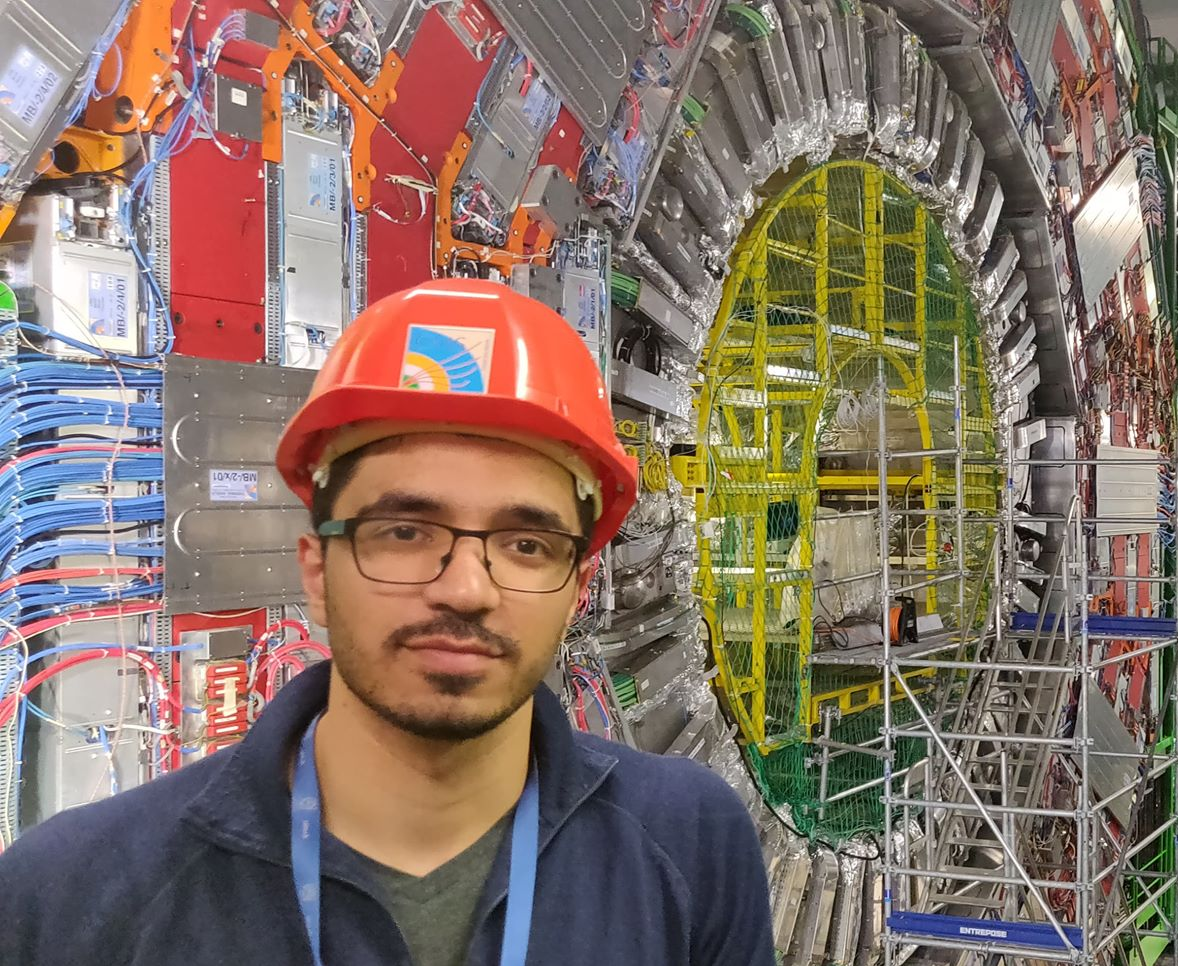
\includegraphics[width=0.8\textwidth]{Billeder/mig.png}
\end{figure}
\end{minipage}
%--------------------------------------------------------------------
\section*{Hvem er jeg?}\vspace{-2.7mm}
\rule{0.7\textwidth}{0.5pt}\vspace{\VRuleDistSmall}

Jeg er en ung maskiningeniørstuderende, som til dagligt arbejder som praktikant ved \textit{Den Europæiske Organisation for Højenergifysik (CERN)} i Schweiz. Jeg studerer til diplomingeniør i maskinteknik på \textit{Ingeniørhøjskolen Aarhus Universitet}. Jeg er en dygtig, ambitiøs og målrettet studerende, som sætter sin uddannelse og fremtidsmuligheder i allerhøjeste sæde. \vspace{\VSecSpace}
%--------------------------------------------------------------------
\section*{Baggrund}\vspace{-3mm}
\rule{1\textwidth}{0.5pt}\vspace{\VRuleDistSmall}

Jeg opdagede min interesse for det tekniske og anvendte naturvidenskab på gymnasiet. Min dengang nyopdagede interesse bidrog til stiftelsen af en ambition, som jeg hårdnakket har fulgt til og med den dag i dag; nemlig at beskæftige mig med ingeniørvidenskaben internationalt ved at tage på et udvekslingsophold i et ingeniørteknisk, førende land. I den anledning skal jeg til efteråret 2019 på udveksling på mit sjette semester i \textit{Nanyang Technological University (NTU)} - ét af Asiens og verdens førende, tekniske universiteter. Dette betragter jeg som en unik og enestående mulighed for min videre færd som maskiningeniør. Opholdet har en varighed af fem måneder i perioden {\Fra-\Till}. \vspace{-11mm}
%--------------------------------------------------------------------
\section*{Formål}\vspace{-3mm}
\rule{1\textwidth}{0.5pt}\vspace{\VRuleDistSmall}

I anledning af mit udlandsophold på NTU, ønsker jeg at søge et legat hos \textit{\FondNavn}, som blandt andre områder, \Aarsag. Det er en nødvendighed, at jeg søger et legat, idet de daglige leve- og boligomkostninger, i Singapore er skyhøje. Men jeg forventer et enormt udbytte af mit ophold, da det muliggøre, at jeg kan tage kurser, som ellers ikke er mulige at få på \textit{Aarhus Universitet}. Jeg har en ambition om at arbejde med maskiner drevet af kunstig intelligens. De nødvendige fag, til at komme ind på denne retning, kan jeg få på NTU. På nuværende tidspunkt mangler jeg netto \underline{\Beloeb kr. } i mit budget (Jf. vedlagte budget), hvori der også indgår udgifter til kulturelle oplevelser. Vigtigheden af dette vil jeg ikke undervurdere, da Singapore er et smeltedigel af de kulturer som omkranser landet, som bør opleves på nært hold. Jeg forventer ikke, at legatet dækker hele mit underskud, men jeg vil værdsætte den mindste smule støtte. \vspace{\VSecSpace}
%--------------------------------------------------------------------
\section*{Hvorfor mig?}\vspace{-3mm}
\rule{1\textwidth}{0.5pt}\vspace{\VRuleDistSmall}

Jeg har gennem hele min studietid arbejdet hårdere end nogen af mine medstuderende, for at sikre min plads på et af verdens førende universiteter. Derfor besidder jeg på nuværende tidspunkt et karaktergennemsnit på \avgKar, som jeg kan høste gevinsten af nu. Jeg forventer, at et udlandsophold på NTU styrker mig fagligt og mentalt; jeg vil stå som en faglig stærkere maskiningeniør ved, at tilegne mig erfaringer og kompetencer indenfor kendskabet til og anvendelsen af kunstig intelligens, som jeg en skønne dag kan anvende i Danmark. Derudover kommer jeg til at lære, at begå mig i et fremmede land og studerer i et internationalt miljø, som vil bidrage til etableringen af et nyt internationalt netværk af ligesindede ingeniører, som kan støtte mig i fremtiden. Foruden faglige kompetencer er forandringsparathed, forandringsvillighed, mentalt robusthed og internationalt 'flair' kernekompetencer, som enhver kommende maskiningeniør bør besidde - især i en verden som i stigende grad globaliseres. Disse kompetencer forventer jeg at tilegne mig, gennem et udlandsophold.

Jeg håber, at I vil tage min anmodning til efterretning og jeg ser frem til at høre fra Jer!
\end{document}

